\documentclass[a4paper,fleqn]{cas-sc}
\usepackage{amsmath,amssymb,amsfonts}
\usepackage{booktabs}
\usepackage{tikz}
\usetikzlibrary{shapes.geometric,arrows.meta,positioning}
\usepackage[authoryear,longnamesfirst]{natbib}
\begin{document}
\RenewDocumentCommand{\printorcid}{}{} % double-blind: suppress empty orcid(s) label
\let\WriteBookmarks\relax
\def\floatpagepagefraction{1}
\def\textpagefraction{.001}

\shorttitle{Evaluating LLM-Based Credit Rating Systems}
\shortauthors{Anonymous}

\title[mode=title]{Evaluating LLM-Based Credit Rating Systems: A Pre-Registered Specification-Curve Analysis}

\author[1]{Anonymous}

\affiliation[1]{organization={Author affiliations withheld for double-blind review}}

\begin{abstract}
Large language models (LLMs) are increasingly used to support credit assessments, but it is unclear
whether elicitation choices merely reveal a stable credit view or shape the rating. Using a pre-registered
specification-curve design that holds fundamentals fixed while varying how the assessment is elicited, we
evaluate 45 credit-health profiles across 32 specifications and three seeds (4{,}320 credit-rating
elicitations), drawn from a pre-registered 90-item battery and a balanced grid of model version,
temperature, prompt paraphrase, output format, few-shot exemplars, and presentation over two providers,
benchmarked to Altman Z$''$. Our estimand is stability,
not accuracy. Under a descriptive main effects decomposition, no controllable axis exceeds about 5\% of
rating variance, and pure run-to-run variation accounts for about 8\%; instability persists on the
temperature-0-honored subgrid (single provider,
temperature 0; permutation $p=0.0005$). Cross-specification agreement remains low at all resolutions:
unweighted Fleiss' $\kappa$ reaches at most 0.49 at the investment-grade/high-yield split, where 25.2\% of
matched pairs disagree, and switching or pooling providers does not remove it. Specification variation is
also observed in 31 perturbed and fingerprint-screened real issuers. A post-hoc check does not detect attenuation on flagship
models, and specification sensitivity is also observed in an open-weight reasoning model. We frame the
elicitation specification as a
model-risk parameter and develop a specification-instability score that predicts held-out instability
(ROC-AUC 0.94; 0.70 on real issuers), a lightweight, ground-truth-free control.
\end{abstract}

\begin{highlights}
\item In the evaluated systems, prompt and model choices move $\sim$25\% of AI credit ratings across the IG/HY line.
\item Descriptive main-effects decomposition: no single elicitation axis accounts for > $\sim$5\% variance. Pure seed noise is $\sim$8\%.
\item Instability persists on the temperature-0-honored subgrid (one provider, temperature 0).
\item Unweighted cross-specification agreement stays modest (Fleiss $\kappa\le0.49$).
\item Score validated on held-out specs (ROC-AUC 0.94) gives a candidate operational model-risk control.
\end{highlights}

\begin{keywords}
large language models \sep credit ratings \sep specification-curve analysis \sep model risk \sep reproducibility \sep investment grade
\end{keywords}

\maketitle

\section{Introduction}
Large language models (LLMs) are increasingly used as an analytic tool in finance, including for
financial-statement interpretation, risk assessment, investment recommendations, and credit analysis
\citep{hens2025risk}. In such applications a user usually provides financial information and asks
the model to make a judgment such as a credit rating, risk category, or trading recommendation. Implicit
in such use is the presumption that the model has a sufficiently stable underlying assessment, and that
reasonable changes to the phrasing of the question simply reveal that assessment. If this assumption is
correct, then choices such as prompt wording, output format, sampling temperature, or model provider are
mostly procedural. If it does not hold, then these choices are embedded in the measurement process
itself.

This distinction is of particular importance for credit evaluation. Credit ratings are categorical
decisions with economically important cut points. The investment-grade/high-yield split influences index
eligibility, ratings-based investment mandates, treatment of collateral, covenant provisions, cost of
financing, and regulatory capital. A model that reaches different assessments because the same financial
information is presented under a different but defensible elicitation specification can lead to materially
different downstream decisions even when the underlying firm fundamentals are unchanged. In our
experiments, around 25\% of matched elicitation pairs place the same credit profile on opposite sides of
the investment-grade/high-yield boundary. The key question we ask is therefore not whether an LLM can
produce a plausible credit rating, but whether the rating is sufficiently stable when reasonable
elicitation choices change.

Prompt sensitivity and run-to-run variability in LLMs have been well documented in computer science
\citep{atil2024nondeterminism,kaplan2020scaling}, and recent work has shown related variability in
LLM-generated financial recommendations \citep{chon2025variability}. But three questions remain
unresolved for high-stakes credit applications. First, it is unclear how large this
instability is in the units used by credit practitioners, rather than generic measures of textual
variation. Second, the variation observed may be due to a small number of controllable design choices,
in which case the instability could be mitigated through an appropriate choice of prompt or model
configuration, or it may signal a broader noise floor that persists across the elicitation process. Third,
evaluation using real firms poses a further challenge: general-purpose LLMs may recognize issuers from
publicly available financial information, making it hard to distinguish independent credit assessment
from memorized issuer knowledge.

We address these questions using a pre-registered specification-curve design based on the
multiverse-analysis literature \citep{simonsohn2020specification,steegen2016multiverse}.
Specification-curve analysis considers a single defensible analytical pipeline as a member of a larger
family of reasonable specifications and tests whether the substantive result depends on the particular
choice. Related approaches have been used to study researcher degrees of freedom and annotation
variability \citep{camuffo2026variance}. We extend this logic to machine elicitation, where the
elicitation specification is varied systematically while the financial information and the underlying
task are held fixed. The distribution of ratings obtained is a direct measure of the dependence of the
machine-generated credit opinion on the way it is asked.

This paper has two co-equal contributions: an \emph{elicitation-reliability evaluation framework} that
measures how LLM-based credit ratings depend on the linguistic and procedural specification, and a
\emph{candidate operational model-risk control} derived from it. In particular we (i) quantify the
sensitivity of machine-generated credit ratings to the elicitation specification and decompose the
rating variation into firm, elicitation-axis, provider-by-item, pure seed, and other unexplained
components; (ii) test the persistence of the instability under two natural remedies, the temperature-0-honored
setting and provider selection, and across rating resolutions from the full letter scale to the
investment-grade/high-yield split; (iii) translate the instability into the decision-relevant unit of
investment-grade/high-yield boundary migration;
(iv) explore external validity descriptively on a perturbed real-issuer arm that first demonstrates
issuer-recognition risk and then mitigates exact-figure recognition through scaling and fingerprint
screening; and (v) develop a candidate operational model-risk control, a
\emph{specification-instability score} with pseudocode, a governance workflow, and a per-issuer cost
model, and validate that it predicts held-out instability (ROC-AUC 0.94). The diagnosis and the control
are co-equal contributions: the first quantifies the problem, the second gives practitioners a
ground-truth-free instrument to manage it.
The main experiment fixes 90 items and pre-registers a grid of elicitation choices, model version,
temperature, prompt paraphrase, output format, few-shot exemplars, and answer presentation, evaluated
across two providers over three repeated seeds (8{,}640 elicitations). The credit-health profiles rest on
a pre-specified Altman Z$''$ accounting-based benchmark \citep{altman1968}, which provides a fixed,
independently computable reference while the elicitation specification varies; our estimand is therefore
not rating accuracy but \emph{stability across specifications}.

\section{Related work}
\subsection{Prompt sensitivity and non-determinism in large language models}
Large language models are built on transformer-based foundation models, and their output depends not only
on the information provided to them but also on how that information is elicited
\citep{vaswani2017attention,devlin2019bert,bommasani2021foundation}. Prior work has demonstrated that
semantically irrelevant or substantively minor changes to prompt construction, such as paraphrasing,
answer format, ordering of options, and sampling configuration, can produce materially different outputs
even when the underlying task is unchanged \citep{atil2024nondeterminism,sclar2024formatspread}.
Non-determinism can also be observed in settings intended to produce deterministic responses
\citep{atil2024nondeterminism}.

These results pose a significant measurement challenge for empirical applications of LLMs. If conclusions
are sensitive to a single wording of a prompt, then an observed model response could be an artifact of
the elicitation specification rather than a stable underlying assessment. \citet{mizrahi2024multiprompt}
demonstrate how single-prompt evaluation can produce fragile conclusions and argue for evaluation across
multiple prompt formulations. In finance, \citet{chon2025variability} likewise find large variation in
stock recommendations produced by LLMs depending on the prompting and model choice.

\subsection{Uncertainty quantification for LLM outputs}
A parallel literature seeks to quantify how confident a model's output is. Self-consistency samples a model
repeatedly and aggregates by majority vote, improving reasoning accuracy and exposing answer dispersion
\citep{wang2023selfconsistency}. Semantic-entropy methods cluster semantically equivalent generations and
measure entropy over meanings to detect unreliable answers \citep{kuhn2023semantic}. Others elicit
confidence directly, teaching models to verbalize calibrated uncertainty \citep{lin2022teaching} or
probing whether models ``know what they know'' \citep{kadavath2022language}. These methods largely target
open-ended generation and token-level or free-text confidence. Our specification-instability score is a
complementary uncertainty measure aimed at a \emph{categorical decision}: rather than sampling one prompt
many times or reading token probabilities, it measures dispersion of the decision class across a fixed set
of defensible elicitation specifications, requires no ground truth or model internals, and reports directly
in the units of the downstream decision (for example, the IG/HY boundary).

\subsection{Multiverse analysis and specification curves}
Empirical results often depend on a set of reasonable analytical choices rather than a single, uniquely
correct specification. The problem has been described as the ``garden of forking paths,'' in which
several defensible decisions can lead to different reported results even in the absence of intentional
specification search \citep{gelman2013garden,simmons2011false}. Multiverse analysis and
specification-curve analysis tackle this problem by assessing the effect across a specified set of
reasonable analytical specifications rather than a single chosen pipeline
\citep{steegen2016multiverse,simonsohn2020specification}.

Specification-curve analysis is particularly useful when the emphasis is on how sensitive a result is to
the choices made by the researcher. The approach examines the distribution of outcomes over the entire
set of defensible specifications, rather than asking whether a given specification leads to a desired
outcome. Similarly, \citet{camuffo2026variance} introduce a variance-aware approach for
LLM-assisted management annotation, underlining the importance of accounting for the variability
introduced by machine-generated annotations.

We extend this framework to LLM elicitation. We treat each combination of the model and the prompting
choices as one specification, while holding the financial information provided to the model fixed. We
treat the LLM as the estimator under study, and the specification curve that arises
measures the degree to which the inferred credit assessment varies solely due to reasonable choices in
how that assessment is solicited.

\subsection{Large language models for finance, credit, and supervision}
LLMs are increasingly employed for financial tasks that were previously the preserve of specialist
judgment, traditional statistical models, or structured quantitative systems. General-purpose
\citep{brown2020gpt3,ouyang2022instruct,achiam2023gpt4} and finance-specific
\citep{wu2023bloomberggpt,xie2023pixiu} language models have been evaluated for
return prediction \citep{lopezlira2023chatgpt}, analysis of central-bank
communication \citep{hansen2024fedspeak}, risk profiling \citep{hens2025risk}, banking supervision
\citep{garciallorente2026banking}, and credit-rating prediction \citep{drinkall2025forecasting}.

Much of this literature evaluates \emph{capability}: whether an LLM can extract useful financial
information, produce accurate forecasts, classify firms, or approximate expert judgments. For instance,
recent work on credit-rating forecasting compares generative LLMs with established predictive approaches
and finds that conventional methods can retain an accuracy advantage \citep{drinkall2025forecasting}.
These studies concern whether the model performs the task well.

Our question comes before that comparison. An LLM-generated credit assessment should be sufficiently
reproducible under reasonable elicitation choices to be interpretable as a meaningful measurement. A
model can appear accurate under one prompt and output a materially different rating under another equally
defensible prompt. We therefore emphasize \emph{stability versus capability}: whether the credit opinion
itself is unchanged when the information being evaluated is unchanged but the elicitation specification
differs.

\subsection{Credit ratings, economic consequences, and model risk}
Quantitative credit-risk assessment has a long history. Altman's bankruptcy-prediction framework
\citep{altman1968} and later probabilistic approaches such as Ohlson's model \citep{ohlson1980} showed
that accounting information contains systematic signal about corporate financial distress. Credit ratings
encode economically relevant differences across firms, and disagreement among human rating agencies has
been studied as a meaningful feature of the credit-rating process itself
\citep{cantorpacker1997,kligersarig2000,tang2009}.

Rating stability matters because shifts in rating categories can influence financing terms and
institutional choices. Rating differences are associated with borrowing costs and
market pricing \citep{kligersarig2000,tang2009,cornaggia2018}, and migration across the
investment-grade/high-yield boundary can have particularly important implications for investment
mandates, portfolio composition, and capital treatment. On the regulatory side, the Basel standardized
approach maps external credit assessments into risk weights for capital calculations
\citep{bcbs2019cre20}, and supervisory exercises have documented considerable dispersion in risk-weighted
assets even for common portfolios \citep{bcbs2013rcap}.

These concerns connect LLM elicitation to the broader literature on model risk. Under supervisory
guidance, models must be validated, their limitations understood, and the uncertainty in their outputs
appropriately characterized \citep{srletter2011}. If the elicitation specification for an LLM-generated
credit rating changes the rating materially, then the specification itself becomes part of the model-risk
environment. Our work ties these literatures together by directly measuring that instability and
quantifying it both through statistical disagreement and through investment-grade/high-yield rating
migration, the decision-relevant unit of the categorical credit limit.

\section{Results}
The pre-registered design assesses the stability of ratings across two providers (OpenAI and Google),
each evaluated at a current and a prior model snapshot (four snapshots in total), giving balanced
coverage across providers, versions, and the elicitation axes. Exact snapshot identifiers are listed in
the Methods (Table~\ref{tab:models}).

\subsection{Sources of rating variation}
We first consider the source of variation in the machine-generated credit rating. An
analysis-of-variance decomposition of the full letter-rating rank (ordinary least squares with Type-II
sums of squares) attributes variance to the firm profile, individual elicitation-design axes, the
provider-by-item interaction, and a residual term (Table~\ref{tab:var}).

As expected, the firm profile explains most of the observed variance, about 65\% (95\% CI 54--72\%),
indicating that the models respond strongly to differences in the underlying financial information. But
the remaining variation is important because the financial information is constant within each item. No
individual controllable elicitation choice explains more than about 5\% of rating variance; the largest
measured design-axis contribution is answer presentation ($\sim$4.6\%, descriptive, under the assumed
main-effects model), and the model-provider main effect contributes only $\sim$0.3\%, with a
provider-by-item interaction of $\sim$1.4\%. The OLS residual
is $\sim$25\%. Because a raw residual can conflate genuine run-to-run randomness with structure the model
omits, we separate the two: \emph{pure within-cell seed variation}, the variance across the three seeds
of each identical item$\times$specification cell, accounts for only 8.1\% of total variance (95\% CI
6.4--10.8\%), leaving the remaining $\sim$17\% as variation not explained by the main-effects model.
That part of the residual is not identified as to source under this resolution-limited D-optimal design
(see Limitations): it may combine real unmodeled interactions with main effects aliased into two-factor
interactions---so we interpret it descriptively instead of attributing it to structured sensitivity.
Run-to-run sampling noise is a real but minor part of the residual.

We report the variance the
elicitation axes explain under three alternatives (Table~\ref{tab:varrange}): a main-effects-only model,
a model adding all two-way interactions, and an issuer-out-of-sample regularized version of the latter.
The apparent explained variance is dependent on the modeling choice, but is low for all three
($R^2$ between $0.08$ and $0.12$), and the in-sample gain from interactions does not fully generalize out
of sample, confirming that individual-axis attribution is not identified and that the decomposition should
be read in a descriptive way.

These results indicate that specification sensitivity is not concentrated in a single elicitation choice
that could be avoided by simply selecting a preferred prompt, format, or provider. Instead, the observed
instability is spread across the elicitation process.

The same pattern appears in the specification curve (Fig.~\ref{fig:speccurve}). The three seeds are
pooled, and each point is a pre-registered specification, sorted by how consistently it recovers the
constructed Altman Z$''$ design labels. Because the profiles were constructed to satisfy those strata,
we interpret this panel as a diagnostic of design-label recovery, not external credit-rating accuracy.
Even when the basic firm profiles are the same, label recovery varies quite a bit across
defensible specs: specs split approximately 56/44 around the pre-registered majority
threshold. Thus, the specification curve shows that conclusions drawn from a single
elicitation configuration do not necessarily generalize to other plausible configurations.

\begin{figure}[t]\centering
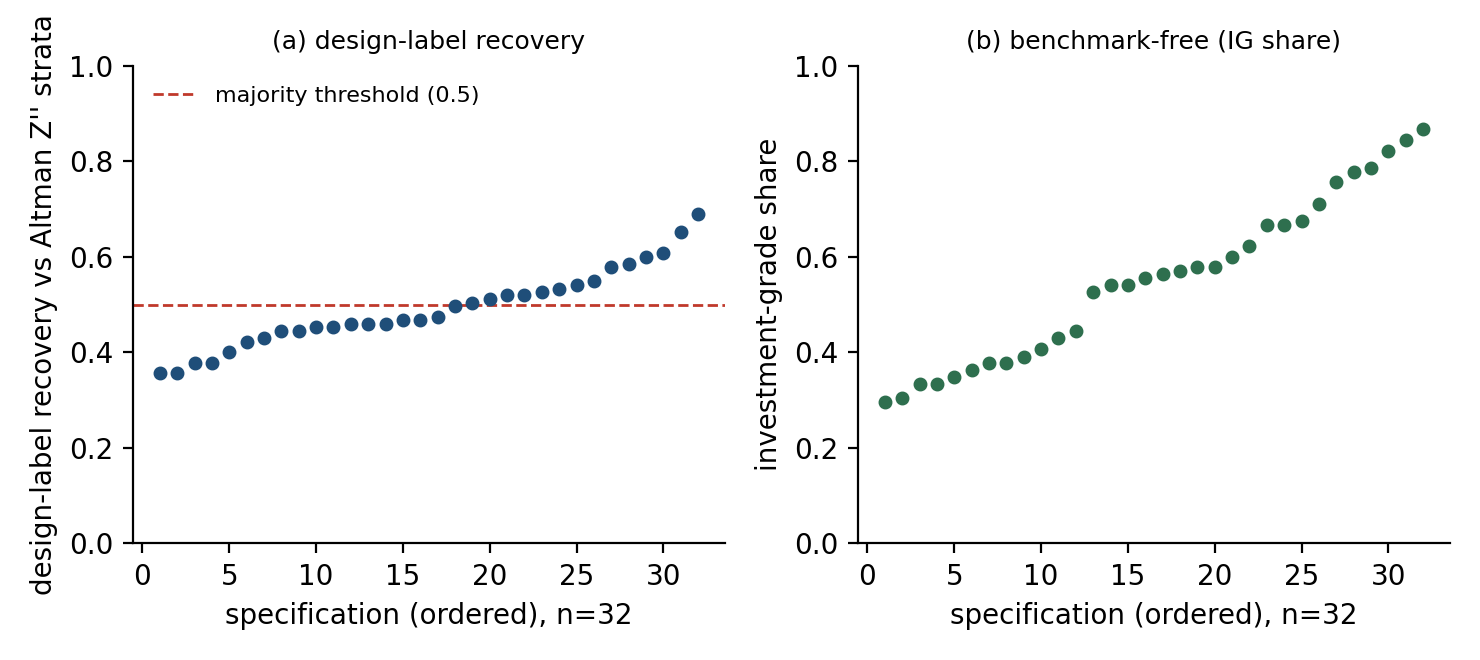
\includegraphics[width=0.92\linewidth]{fig_spec_curve.png}
\caption{Specification curves of the machine credit rating; each point is one pre-registered
specification (three seeds pooled), specifications sorted independently in each panel. \textbf{(a)}
Design-label recovery: agreement with the constructed Altman Z$''$ strata (the profiles were built to
satisfy these strata, so this is label recovery, not external accuracy) the specs split about
56/44 around the majority line. \textbf{(b)} Benchmark-free: the
share of a specification's credit elicitations rated investment grade, which needs no ground truth and
ranges widely across specifications, direct evidence that the verdict, not merely its accuracy, moves
with the elicitation. This is the multiverse the method is named for.}
\label{fig:speccurve}
\end{figure}

\begin{table}[t]\centering
\caption{Variance shares of the machine credit letter-rank (OLS decomposition with Type-II ANOVA;
$n=45$ items). The residual is split into pure within-cell seed variance and other unexplained variance.
Confidence intervals (profile-clustered bootstrap, 95\%) are reported only for the item and pure-seed components; the per-axis shares are descriptive and carry no intervals.}\label{tab:var}
\begin{tabular}{lr}\toprule
Component & Variance share \\\midrule
Item (firm profile) & 64.9\% (53.9--72.3\%) \\
Residual (total) & 25.2\% \\
\quad --- pure within-cell seed variation & 8.1\% (6.4--10.8\%) \\
\quad --- other unexplained (unmodeled interactions) & $\sim$17\% \\
Answer presentation ($A_7$, largest design axis) & 4.6\% \\
Provider $\times$ item interaction & 1.4\% \\
Temperature / prompt paraphrase / few-shot / format / version & $\le$1.0\% each \\
Model provider (main effect) & 0.3\% \\\bottomrule
\end{tabular}

\vspace{3pt}
{\footnotesize\raggedright The item, design-axis, provider$\times$item interaction, and residual shares
partition the total variance and sum to 100\% up to rounding; the two indented rows are a decomposition
of the residual, not additional components. Design diagnostics: main-effect columns are near-orthogonal
(maximum off-diagonal correlation $0.062$), while the maximum absolute correlation between main-effect and
two-factor-interaction columns is $0.333$; non-negligible aliasing remains, so per-axis shares are
descriptive, not identified.}
\end{table}

\begin{table}[t]\centering
\caption{Variance in the machine letter rating explained by the elicitation axes under different model
specifications (credit-health task; issuer identity removed to isolate the axes). The estimate is changing
with the model and remains small throughout. This illustrates that per-axis attribution is not identified under the design.}
\label{tab:varrange}
\begin{tabular}{lc}\toprule
Model specification & $R^2$ \\\midrule
Main effects only & 0.083 (in-sample) \\
Main effects $+$ all two-way interactions & 0.119 (in-sample) \\
Regularized two-way (ridge), issuer out-of-sample & 0.101 (5-fold, issuer group) \\\bottomrule
\end{tabular}\end{table}

\subsection{Specification fragility on the temperature-0-honored subgrid}
One explanation of this residual variation is that a provider may not fully honor a requested
temperature of zero. If so, the observed instability might largely reflect stochastic sampling rather
than sensitivity to the elicitation specification per se.

We therefore perform the pre-registered determinism test and restrict the analysis to the
provider-setting combination for which the returned metadata confirm that temperature was honored: Google
at temperature 0. This temperature-0-honored subgrid sharply reduces repeated-call sampling variation but
retains substantial specification dependence. In it, 62.5\% of specifications are on opposite side of the majority
label-recovery threshold, and consistency with the constructed credit-band design labels ranges from 0.36 to
0.69 across temperature-0 prompt configurations.

A one-sided permutation test rejects the null of specification invariance of the \emph{rating} itself.
The test permutes specification-condition assignments across profiles (a null of rating invariance, rather
than permuting accuracy labels), with the statistic the between-specification spread of the item-centred
letter grade. On the temperature-0-honored Google subgrid, the observed spread is $1.59$ notches, versus
a permutation-null mean of $0.18$ notches and standard deviation $0.050$ notches; across $2{,}000$ permutations
none achieved the value observed, giving $p=0.0005$ (specification $\eta^2=0.46$ on the item-centred
rating, a specification-level aggregate not comparable to the individual-rating partition of
Table~\ref{tab:var}). Holding temperature at 0 thus removes much of the run-to-run jitter but does not eliminate
sensitivity to prompt and presentation choices; indeed, the specification-curve flip share within the
temperature-0-honored subgrid is higher than the pooled estimate. The instability therefore cannot be ascribed
solely to stochastic sampling, consistent with the variance decomposition, in which pure seed variation
is a minority of the residual.

\subsection{Agreement within and between providers}\label{sec:agreement}
The small provider main effect might suggest that provider choice does not matter much. Direct agreement
comparisons reveal a more complex pattern.

Within-provider agreement is consistently higher than cross-provider agreement. Within a single provider,
82.5\% of identical firm profiles agree at the three-way credit-band level, but only 64.4\% agree across
the two providers. At the full letter-rating level, agreement across providers falls to 11.1\% from
30.4\% within providers.

These findings are consistent with the variance decomposition. The two providers respond differently to
specific firm profiles, creating a provider-by-item interaction. The interaction does not appear to
reflect a constant directional shift in ratings; a simple global adjustment does not allow one provider to
be characterized as systematically more conservative or more generous than the other. The disagreement is
issuer-specific.

This distinction is important operationally. Changing vendors does not provide a predictable correction
to the rating of a specific firm, and aggregating outputs across vendors does not remove the underlying
specification dependence. Vendor diversification therefore does not resolve the conceptual measurement
problem or the need to characterize uncertainty across elicitation specifications.

\subsection{Stability across rating resolutions}
Credit ratings are inherently hierarchical. A model may not reproduce an exact letter grade yet still
express a stable broader assessment. We therefore assess cross-specification agreement as we move from
the full 21-grade letter-rating scale to notch categories, three broad credit bands, and the binary
investment-grade/high-yield distinction (the deterministic mappings are given in Table~\ref{tab:map}).

Agreement improves as the scale is coarsened but does not become fully stable. Raw cross-specification
agreement is approximately 17\% at the letter level, 36\% at the notch level, 68\% for the three-way
credit band, and 75\% for the investment-grade/high-yield split. Equivalently, matched elicitation pairs
disagree in about 83\%, 64\%, 32\%, and 25\% of comparisons, respectively (Fig.~\ref{fig:ighy}).

The same conclusion follows from chance-corrected agreement. Fleiss' $\kappa$ is 0.10 at the full letter
scale, 0.21 at the notch level, 0.43 for the three-way band, and reaches a maximum of only 0.49 for the
investment-grade/high-yield split (Fig.~\ref{fig:kappa}). No evaluated rating resolution meets the
conventional threshold for substantial agreement ($\kappa=0.60$) under unweighted scoring.

Because unweighted $\kappa$ on 21 ordinal grades penalizes an AAA-versus-AA$+$ disagreement as heavily
as AAA-versus-C, we also report ordinal-weighted agreement on the letter-rank scale: Krippendorff's
$\alpha$ is 0.44 under linear weighting and 0.65 under quadratic weighting. Fine-grained disagreement is
therefore concentrated among adjacent grades. This weighting, however, cannot apply to the binary
investment-grade/high-yield decision, where the only two categories are maximally distant and 25.2\% of
matched pairs still cross the boundary; the decision-relevant instability is unaffected by how ordinal
proximity is credited.

The instability is not caused by the models collapsing to a narrow set of central ratings. All 21 letter
grades are used across the experiment (pooled scale-usage entropy 3.89 of a maximum 4.39 bits). This
spread is not merely across firms: the mean \emph{per-firm} rating entropy is 2.85 bits, so a single
firm's rating is itself distributed over roughly seven effective grades as the specification varies. The
models therefore use the available rating scale extensively but do not reproduce the same assessment
consistently across specifications.

The most economically consequential result appears at the coarsest resolution. Even when all finer
distinctions are dropped and only the investment-grade/high-yield classification is retained, 25.2\% of
matched elicitation pairs place the same firm profile on opposite sides of the boundary. Coarsening
reduces specification sensitivity but does not eliminate it.

This boundary instability is not uniform across the credit spectrum. The per-comparison IG/HY flip is 13.0\% among benchmark-SAFE profiles, rises to
35.5\% among benchmark-WATCH profiles adjacent to the boundary, and is 27.1\% among benchmark-DISTRESS
profiles. Because the battery is balanced across the three strata by construction (15 profiles each), the
pooled 25.2\% is the average over strata rather than an artifact of oversampling near-boundary firms.
The flip is elevated in the near-boundary WATCH stratum, but when we treat distance from the boundary
continuously it does not decline monotonically with that distance (Spearman between per-item flip and
$|$Z$''-2.60|$ is $-0.05$), so the instability is broadly distributed across the credit spectrum rather
than confined to a narrow near-boundary band.

\begin{figure}[t]\centering
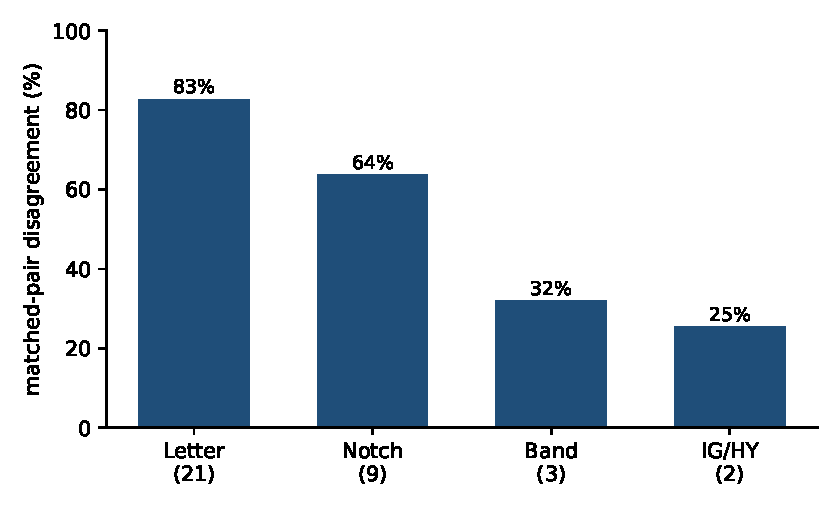
\includegraphics[width=0.66\linewidth]{figure1_ighy.pdf}
\caption{Share of matched elicitation pairs whose credit verdicts differ, by rating granularity, where
the two elicitations of a firm may differ on any grid axis (provider, model version, temperature,
paraphrase, format, few-shot, presentation) and seed. Even at the coarse investment-grade/high-yield
split, the most consequential line in credit, about 25\% of matched pairs disagree.}\label{fig:ighy}
\end{figure}
\begin{figure}[t]\centering
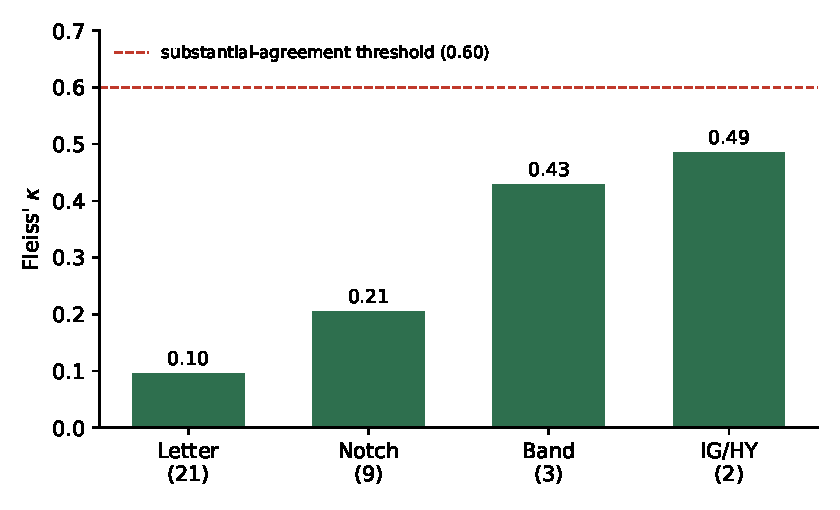
\includegraphics[width=0.62\linewidth]{figureA_kappa.pdf}
\caption{Chance-corrected cross-specification agreement (unweighted Fleiss $\kappa$) by granularity;
agreement peaks at 0.49 on the IG/HY split and no resolution reaches the $\kappa=0.6$ substantial
threshold under unweighted scoring. Ordinal weighting raises letter-scale agreement (Krippendorff's
$\alpha=0.65$ quadratic), but the binary IG/HY flip is unaffected by weighting.}
\label{fig:kappa}
\end{figure}

\subsection{Migration from investment-grade to high-yield}
Statistical disagreement is economically important when alternative specifications produce decisions on
opposite sides of material credit boundaries. The observed rating instability is understood as the
decision-relevant unit of investment-grade/high-yield migration.

For each credit-health profile we draw two elicitations from its observed specification distribution,
allowing the pair to differ on any elicitation axis and on seed. We then compute, for each firm, the
probability that the two resulting ratings fall on opposite sides of the investment-grade/high-yield
boundary, and average across profiles. This per-comparison flip probability is one minus the
Gini--Simpson concentration of the firm's binary IG/HY outcomes.

This yields an investment-grade/high-yield flip rate of 25.2\% (95\% CI 19.7--31.2\%): about a quarter of
matched ratings for the same underlying credit profile disagree on which side of the investment-grade
boundary the profile falls (Table~\ref{tab:frag}). Because the boundary governs index eligibility,
mandate constraints, collateral treatment, and cost of financing, migration of this magnitude driven
solely by the elicitation specification is economically consequential.

\begin{table}[t]\centering
\caption{Fragility in decision and rating units. Parenthetical values are 95\% confidence intervals
(profile-clustered percentile bootstrapping)}\label{tab:frag}
\begin{tabular}{lr}\toprule
Quantity & Result \\\midrule
Specifications flipping majority credit \emph{band} verdict (pooled / determ.) & $\sim$56\% / 62.5\% \\
Design-label recovery range, temperature-0-honored subgrid & 0.36--0.69 \\
Permutation test, temperature-0-honored subgrid (rating-invariance null) & $p=0.0005$ (2{,}000 perms) \\
Within- vs cross-provider agreement (band / letter) & 82.5/64.4 $\cdot$ 30.4/11.1 \\
Max chance-corrected agreement (Fleiss $\kappa$, IG/HY) & 0.49 (no scale $\geq0.6$) \\
Per-comparison IG/HY boundary flip & 25.2\% (95\% CI 19.7--31.2\%) \\\bottomrule
\end{tabular}\end{table}

\subsection{Illustrative check on perturbed and fingerprint-screened real issuers}\label{sec:realarm}
The constructed battery provides the controlled context in which to identify elicitation instability, but
a key external-validity concern is whether similar behavior appears for real firms. Direct evaluation on
real issuers raises a further methodological problem: an LLM may recognize a company from publicly
available financial figures even when the company name is removed.

We test this possibility, and then use the real issuers as a descriptive external check. When presented with
anonymized but otherwise unchanged financial profiles, Gemini-Flash correctly identifies about 22\% of
the selected mid-cap issuers from their financial numbers alone. This shows that anonymizing the issuer
name does not guarantee that an LLM makes an independent credit assessment rather than relying on
memorized issuer information.

The pre-registered fingerprinting gate lowered the issuer-identification rate from 22\% to 2.9\%, below
the pre-specified 5\% threshold. The retained perturbed firms are then rated on a frozen 12-specification grid
at three seeds, and the constructed battery is re-rated under exactly the same specification grid to
provide a matched comparison.

The real-firm WATCH-stratum flip share is 0.226 (95\% CI 0.147--0.308), relative to 0.318 (95\% CI
0.223--0.406) for the matched constructed battery. The estimated difference is $-0.091$ (95\% CI $-0.213$
to $0.032$; Table~\ref{tab:realarm}), not statistically distinguishable from zero. We treat this arm as an
illustrative external-validity check, presented descriptively: specification variation is also observed
in the perturbed and fingerprint-screened real issuers under the same elicitation conditions, but the small sample (16 real, 15
battery WATCH observations) cannot establish that its magnitude equals the constructed battery's.

We also discuss the relevant concern that the perturbation-and-screening procedure or the selection of the external
benchmark may be driving the result. First, the per-issuer scaling is uniform, meaning all financial
ratios and the Altman Z$''$ are invariant by construction (Z$''$ transformed-vs-original correlation
$1.000000$; $100\%$ of issuers retain their original stratum), and the realized scale factors, which span
the full pre-registered $[0.6,1.7]$ range across the 31 issuers, show no association with per-issuer
instability or rating level (Spearman $-0.035$, permutation $p=0.85$); a single draw per issuer means
scale is confounded with issuer identity, so we read this as within-support evidence rather than a
scale-invariance proof. Second, using the disclosed agency ratings as an external benchmark not used to
construct the profiles, per-specification credit-band accuracy on the real issuers (the SAFE and WATCH
strata, i.e.\ 30 of the 31 issuers; the single DISTRESS issuer is a singleton excluded from this
three-band accuracy comparison) ranges from $42.2\%$
to $61.1\%$ across the 12 specifications (mean $53.7\%$); an issuer-preserving permutation test (specification
labels permuted within issuer) finds this between-specification spread beyond chance ($p=0.021$). Specification
sensitivity is therefore visible against a genuinely external benchmark, not only against the constructed
labels. Machine-generated credit bands correspond to disclosed agency ratings
about $54\%$ of the time, above the $\sim$33\% expected by chance on 3 bands but far from reliable
accord.

\begin{table}[t]\centering
\caption{Real-firm arm: 31 perturbed and fingerprint-screened business-to-business issuers, agency-rating benchmark.
Parenthetical values are 95\% confidence intervals (issuer-clustered percentile bootstrap).}
\label{tab:realarm}
\begin{tabular}{lr}\toprule
Quantity & Result \\\midrule
Fingerprint identification, naive (exact figures) & 22\% \\
Fingerprint identification, after perturbation and screening & 2.9\% \\
WATCH-stratum flip-share, real arm & 0.226 (0.147--0.308) \\
WATCH-stratum flip-share, battery (same 12 specs) & 0.318 (0.223--0.406) \\
Difference (real $-$ battery), 95\% CI & $-0.091$ ($-0.213$, $0.032$) \\
external-benchmark spec. curve, per-spec accuracy range & 42.2--61.1\% (spread perm. $p=0.021$) \\
Interpretation & illustrative external check, presented descriptively \\
Machine band vs.\ disclosed agency rating (descriptive) & 54\% ($\sim$33\% chance) \\\bottomrule
\end{tabular}\end{table}

\subsection{Robustness across model tiers (post-hoc)}\label{sec:tier}
This analysis is \emph{post-hoc}: it was not part of the pre-registered design and was carried out in a
separate run after the confirmatory corpus was frozen, to address the
concern that the instability might be an artifact of the low-cost model tier. We re-ran the frozen
12-specification grid over the 45 credit-health profiles at three seeds using each provider's flagship
model (\texttt{gpt-5.4} and \texttt{gemini-3.1-pro-preview}), and compared it to the nano/flash tier
evaluated on the identical grid. The per-comparison IG/HY flip is 23.6\%
(95\% CI 19.4--27.8\%) on the flagship tier versus 24.7\% (95\% CI 19.1--30.6\%) on nano/flash; the
paired difference is $-1.1$ percentage points (95\% CI $-7.6$ to $+6.0$), not distinguishable from zero
(Table~\ref{tab:tier}). The three-way band flip is likewise statistically indistinguishable
($-5.3$ points; 95\% CI $-11.9$ to $+1.3$). Flagship models are notably more lenient, they assign
investment grade to 79.9\% of elicitations versus 58.6\% at the nano/flash tier, yet are no more
consistent across elicitation choices. We do not detect attenuation of specification sensitivity at the
flagship tier: the paired difference is small and statistically indistinguishable from zero, with a wide
interval ($-1.1$ pp, 95\% CI $-7.6$ to $+6.0$). This is an absence-of-evidence result, not evidence of
absence, and is consistent with the instability being a property of how the categorical judgment is
elicited rather than of model scale.

Two caveats attach to this comparison. First, the pooled figure masks provider heterogeneity: the
flagship IG/HY flip is 26.7\% for OpenAI (versus 17.3\% at the nano tier) but 16.7\% for Google (versus
20.5\%), so the pooled near-equality reflects partial cancellation across providers rather than uniform
stability. Second, the tiers are not perfectly generation-matched on the Google side, no Gemini-3.5 Pro
model exists, so the flagship \texttt{gemini-3.1-pro-preview} is one minor generation behind its
\texttt{gemini-3.5-flash} nano counterpart, whereas the OpenAI pair (\texttt{gpt-5.4} versus
\texttt{gpt-5.4-nano}) is generation-matched. Finally, the flagship models do not recover the built
Altman labels more often despite being easier to meet: flagship design-label recovery is 36.7\% compared to 44.3\% for
nano/flash, so the 21-point investment-grade leniency shift reflects a more permissive rating posture,
less close correspondence with the constructed labels.

\begin{table}[t]\centering
\caption{Model-tier robustness (post-hoc; not pre-registered): per-comparison flip share on the same
frozen 12-specification grid ($45$ credit-health items, three seeds). Parenthetical values are 95\%
profile-clustered bootstrap confidence intervals. The difference is paired by item.}
\label{tab:tier}
\begin{tabular}{lccc}\toprule
Metric & Nano/flash & Flagship & Difference (95\% CI) \\\midrule
IG/HY flip (pooled) & 24.7\% (19.1--30.6) & 23.6\% (19.4--27.8) & $-1.1$ ($-7.6$, $+6.0$) \\
\quad IG/HY flip, OpenAI & 17.3\% & 26.7\% & \\
\quad IG/HY flip, Google & 20.5\% & 16.7\% & \\
Three-way band flip & 30.5\% & 25.2\% & $-5.3$ ($-11.9$, $+1.3$) \\\midrule
Design-label recovery vs Altman & 44.3\% & 36.7\% & \\
IG rate (leniency) & 58.6\% & 79.9\% & \\\midrule
\multicolumn{4}{l}{Nano/flash: \texttt{gpt-5.4-nano} + \texttt{gemini-3.5-flash}. Flagship: \texttt{gpt-5.4} + \texttt{gemini-3.1-pro-preview}.}\\
\multicolumn{4}{l}{The pooled IG/HY flip exceeds both per-provider figures because pooling adds cross-provider}\\
\multicolumn{4}{l}{disagreement absent within a single provider (Section~\ref{sec:agreement}).}\\
\multicolumn{4}{l}{Google flagship is one minor generation behind its flash counterpart (no Gemini-3.5 Pro exists).}\\\bottomrule
\end{tabular}\end{table}

\subsection{Model class robustness: a reasoning architecture (post-hoc)}\label{sec:reasoning}
This analysis is \emph{post-hoc}: it was not pre-registered and was collected in a separate run to address
the worry that instability could be resolved by an explicit reasoning pipeline. We ran the frozen
12-specification grid over the 45 credit-health profiles at three seeds on an open-weight model with a
native chain-of-thought, DeepSeek-R1 (via the OpenRouter API; frozen under
\texttt{MANIFEST\_REASONING.sha256}), adding a third model family and reasoning architecture. Because a
single model instantiates the grid, this arm exercises the three non-provider axes (paraphrase, output
format, presentation) and holds the fourth grid axis, provider, constant.

The per-comparison IG/HY flip is 25.5\% (95\% CI 20.9--30.1\%), and the paired difference against the
nano/flash tier is $+0.9$ percentage points (95\% CI $-7.0$ to $+8.8$), indistinguishable from zero
(Table~\ref{tab:reason}). Two design differences qualify the comparison rather than make it strictly
like-for-like: the reasoning arm shows no cross-provider variation (the largest single agreement gap,
Section~\ref{sec:agreement}), and DeepSeek-R1 has a much more skewed marginal, giving
investment grade to only 31.4\% of elicitations, compared with 79.9\% for the flagship tier. We therefore read
the 25.5\% flip as evidence of specification sensitivity within the evaluated reasoning model. In this arm,
we do not detect attenuation of elicitation sensitivity under chain-of-thought reasoning.

\begin{table}[t]\centering
\caption{Reasoning-architecture arm (post-hoc; not pre-registered): per-comparison IG/HY flip on the
frozen 12-specification grid (45 credit-health items, three seeds), and two-provider tiers for
reference. The reasoning arm holds provider constant (single model); the paired difference is item-wise.}
\label{tab:reason}
\begin{tabular}{lcc}\toprule
Tier & IG/HY flip (95\% CI) & IG rate \\\midrule
Nano/flash (two providers) & 24.7\% (19.1--30.6) & 58.6\% \\
Flagship (two providers) & 23.6\% (19.4--27.8) & 79.9\% \\
Reasoning \texttt{deepseek-r1} (single model) & 25.5\% (20.9--30.1) & 31.4\% \\\midrule
\multicolumn{3}{l}{Paired difference, reasoning $-$ nano/flash: $+0.9$ percentage points (95\% CI $-7.0$, $+8.8$).}\\
\multicolumn{3}{l}{Reasoning arm varies three non-provider axes; provider is held constant.}\\\bottomrule
\end{tabular}\end{table}

\subsection{Self-consistency: does aggregation remove the instability? (post-hoc)}\label{sec:selfcons}
This analysis is post-hoc and was not part of the pre-registration. A natural remedy is self-consistency: instead of acting on a single elicitation, query the model under
$k$ defensible specifications and act on the majority vote. We quantify how much this helps by computing,
for each issuer, the residual probability that two independent $k$-of-$n$ majority votes land on opposite
sides of the IG/HY boundary, averaged over issuers, for $k=1,3,5,9,15$ (Fig.~\ref{fig:selfcons}).
Aggregation reduces but does not remove the instability: the residual flip falls from 25.2\% at $k=1$ to
19.4\% ($k=3$), 16.6\% ($k=5$), 13.6\% ($k=9$), and 11.1\% at $k=15$. Even fifteen aggregated
elicitations therefore leave roughly one in nine matched issuer assessments crossing the
investment-grade boundary. Self-consistency is a partial control whose cost grows linearly in $k$; it
motivates reporting the residual dispersion explicitly rather than assuming a single call is
representative, which is the role of the specification-instability score developed next.

\begin{figure}[t]\centering
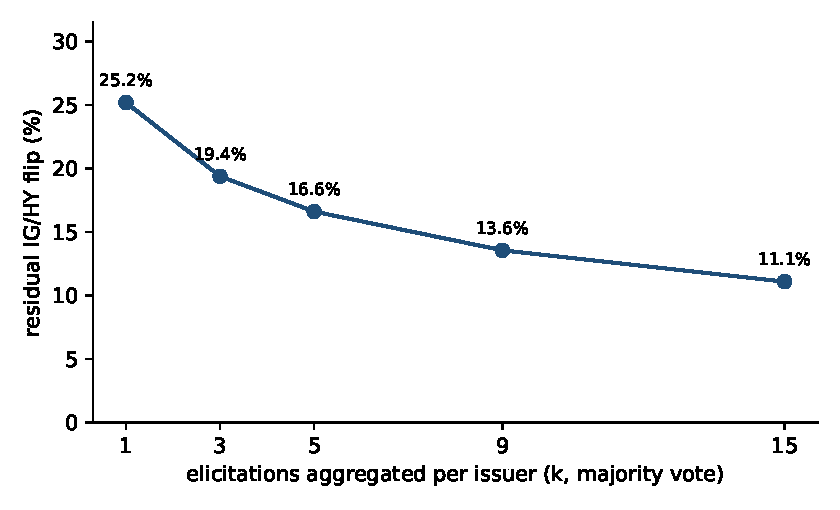
\includegraphics[width=0.62\linewidth]{fig_selfconsistency.pdf}
\caption{Self-consistency curve: residual per-comparison IG/HY flip after aggregating $k$ elicitations
per issuer by majority vote. Aggregation lowers instability with diminishing returns and does not
eliminate it, about 11\% of matched assessments still cross the boundary at $k=15$.}\label{fig:selfcons}
\end{figure}

\section{A specification-instability score for model-risk control}\label{sec:sis}
The diagnosis above is actionable. Because the instability is a property of the elicitation process, it
can be measured at inference time from the model's own outputs and reported alongside every rating,
turning the specification curve from a research diagnostic into an operational model-risk control. This
section defines the control, validates that it predicts held-out instability, and specifies its
deployment cost and governance use.

\subsection{Definition}
For an issuer $x$, fix a small set $S$ of $k$ defensible elicitation specifications and a decision
resolution $g$ (for example, the map from letter grade to the IG/HY class). Query the model once per
specification, map each rating to its decision class, and let $p_{x,c}$ be the fraction of the $k$
elicitations that fall in class $c$. The \emph{specification-instability score} is the Gini--Simpson
dispersion of that distribution,
\begin{equation}
\mathrm{SIS}(x) \;=\; 1 - \sum_{c} p_{x,c}^{2},
\end{equation}
reported alongside the modal rating $\hat{r}(x)=\arg\max_c p_{x,c}$. A score of zero denotes a perfectly
stable, specification-invariant rating; higher values flag issuers whose rating is substantially an
artifact of how the question was asked (the theoretical maximum for a binary decision is $0.5$). The score
requires no ground truth and no access to model internals, so it applies to any API-served model
(Algorithm~1, Fig.~\ref{alg:sis}). The Gini--Simpson form itself is a standard dispersion index; the
contribution here is not a new mathematical index but its use as a candidate operational credit-model-risk control,
its validation on held-out specifications, its governance trigger, and its cost model.

\begin{figure}[t]\centering
\fbox{\begin{minipage}{0.92\linewidth}\ttfamily\footnotesize
\textbf{Algorithm 1.} Specification-instability score and review trigger\\[2pt]
\textbf{input:} issuer $x$; spec set $S$ ($|S|{=}k$); resolution map $g$; model $M$;\\
\phantom{\textbf{input:} }boundary set $B$; tolerance $\tau$\\
1\quad $C \leftarrow [\,]$\\
2\quad \textbf{for} $s$ \textbf{in} $S$:\\
3\quad\quad $r \leftarrow M(x, s)$ \hfill \# one elicitation\\
4\quad\quad append $g(r)$ to $C$ \hfill \# map rating to decision class\\
5\quad $p_c \leftarrow |\{i : C_i = c\}| / k$ \ for each class $c$\\
6\quad $\hat{r} \leftarrow \arg\max_c p_c$; \quad $\mathrm{SIS} \leftarrow 1 - \sum_c p_c^2$\\
7\quad $\mathit{flag} \leftarrow (\hat{r} \in B)$ \textbf{and} $(\mathrm{SIS} > \tau)$\\
8\quad \textbf{return} $(\hat{r},\ \mathrm{SIS},\ \mathit{flag})$
\end{minipage}}
\caption{Specification-instability score and review trigger; ground-truth-free and computable from any
Model served via API. The tolerance $\tau$ is $k$-dependent (the attainable score grid is discrete in $k$);
in deployment it is defined as the ``flag any disagreement'' rule at the chosen $k$ (Section~\ref{sec:sis-val}).}\label{alg:sis}
\end{figure}

\subsection{Post-hoc validation on held-out specifications}\label{sec:sis-val}
This validation is \emph{post-hoc} (it was not part of the pre-registration) and tests generalization
across specifications, not across an external issuer sample. A control is only useful if it predicts
instability it has not seen, so we split the 32 specifications into a 16-specification calibration set and
a disjoint 16-specification validation set, compute $\mathrm{SIS}$ for each issuer on the calibration set
only, and ask whether it predicts that issuer's behaviour on the held-out validation specifications. The
calibration score is strongly rank-correlated with the held-out flip rate (Spearman $\rho=0.89$). Treating
``the issuer's modal IG/HY call flips on at least one held-out specification'' as the event to be flagged
(base rate $0.76$), the calibration score has a ROC-AUC of $0.94$ (profile-clustered bootstrap 95\%
CI $0.86$--$0.99$) and average precision of $0.98$. To rule out sensitivity to a single partition, we
repeat the analysis over 300 balanced random calibration/validation splits: the median AUC is $0.88$
(interquartile range $0.86$--$0.91$; full range $0.73$--$0.98$). The score therefore identifies, from a
handful of elicitations, the issuers whose ratings will prove unstable under specifications not yet
tried; these results support the score as a candidate operational screening control for the evaluated model/specification setting.

We also check whether this generalizes beyond the synthetic battery by repeating the validation on the
31 perturbed and fingerprint-screened \emph{real} issuers (Section~\ref{sec:realarm}), for which the same 12-specification
grid was collected. Splitting those specifications 6/6, the calibration-set score remains predictive of
held-out-specification instability on real firms (ROC-AUC 0.70, issuer-clustered bootstrap 95\% CI
0.51--0.87; Spearman $\rho=0.41$; base rate 0.61). Discrimination is weaker than on the synthetic battery
and the interval is wide, expected given only 31 issuers and a coarser six-specification calibration, but
the score carries a genuine, same-direction signal on real issuers, not only on the constructed profiles.
We nonetheless emphasize that ``external'' here means external \emph{issuers}, not external
specifications; a fully out-of-sample external issuer \emph{population} remains future work. We also
report the recalibration requirement for a new model directly: cross-model transfer of the score is
moderate but inconsistent across model pairs (per-item Spearman between one model's score and another's
ranges from $0.14$ to $0.73$, median $\approx0.45$, and $\approx0.55$ across provider families; the AUC of
one model's score for flagging another's above-median-instability items has median $\approx0.72$). Because
this transfer is too variable to rely on, a new model should be re-scored on the grid rather than reusing
another model's scores, at about \$7.43 per 1{,}000 issuers at $k=9$ on a
nano/flash tier (Table~\ref{tab:cost}).

A practical operating threshold must recognize that at $k=16$ the achievable score values are discrete:
for a binary IG/HY outcome $\mathrm{SIS}$ jumps from $0$ (unanimous) to $0.117$ (one dissenter), with
nothing between. The threshold that maximizes Youden’s $J$ on the held-out split, $\tau=0.08$, therefore
is less than $0.117$ and reduces to a rule that flags any issuer with at least one disagreeing calibration
elicitation, at which held-out precision is $1.00$ and recall $0.88$; we report it as a descriptive
operating point (chosen and evaluated on the same split). Note that it is $k$-dependent (at the recommended
$k\approx9$ the smallest non-zero score is $0.198$). This rule alone would cover some $67\%$ of issuers,
a direct implication of the finding that most issuers disagree on at least one specification; Algorithm~1
therefore refers to issuers with a modal rating close to a decision boundary as well, which roughly halves
the referred set to about $33\%$. The continuous score is used for ranking and triage---its discrimination
(ROC-AUC $0.94$) scored on the full score, not the binary gate---so at finer resolutions than IG/HY it
has many values rather than collapsing to a flag indicating unanimity.

\subsection{Deployment: aggregation level and cost}\label{sec:sis-cost}
The number of elicitations $k$ trades stability against cost. The self-consistency curve
(Section~\ref{sec:selfcons}) shows steeply diminishing returns: the modal call's residual IG/HY flip
falls from 25.2\% at $k=1$ to 13.6\% at $k=9$ and 11.1\% at $k=15$, so a moderate $k\!\approx\!9$ captures
most of the achievable stabilization while still exposing residual dispersion through the score. The cost
is modest and linear in $k$: at $k=9$, scoring one thousand issuers requires about $3.7$ million tokens
and costs roughly \$7 on a nano/flash tier or \$118 on a flagship tier (Table~\ref{tab:cost}). Because the
score is computed from calls the workflow already makes, its marginal cost over simply issuing a rating is
the $k-1$ additional elicitations.

\begin{table}[t]\centering
\caption{Deployment cost of the specification-instability score by aggregation level $k$: cost to score
1{,}000 issuers, from the observed per-call token counts and provider pricing.}\label{tab:cost}
\begin{tabular}{rrrr}\toprule
$k$ & Tokens/issuer & \$/1{,}000 (nano/flash) & \$/1{,}000 (flagship) \\\midrule
1 & 416 & 0.83 & 13.12 \\
3 & 1{,}248 & 2.48 & 39.37 \\
5 & 2{,}080 & 4.13 & 65.61 \\
9 & 3{,}745 & 7.43 & 118.10 \\
15 & 6{,}242 & 12.38 & 196.84 \\\bottomrule
\end{tabular}

\vspace{3pt}
{\footnotesize\raggedright Token counts are the observed per-call means; dollar figures use provider list
pricing accessed August 2026 from the OpenAI and Google API pricing pages and will change as pricing
changes.\par}
\end{table}

\subsection{Governance workflow}\label{sec:sis-gov}
In a model-risk workflow the score sits between the model and the decision (Fig.~\ref{fig:governance}).
Each issuer is elicited $k$ times; the modal rating and its score are recorded; issuers whose modal rating
sits near a consequential boundary (such as IG/HY) \emph{and} whose score exceeds a pre-set tolerance are
routed to human review, while stable issuers pass through. This yields an auditable, ground-truth-free
control that scales with the rating pipeline and directly answers a supervisory model-risk question:
how much of this rating is a property of the firm, and how much of how we asked?

\begin{figure}[t]\centering
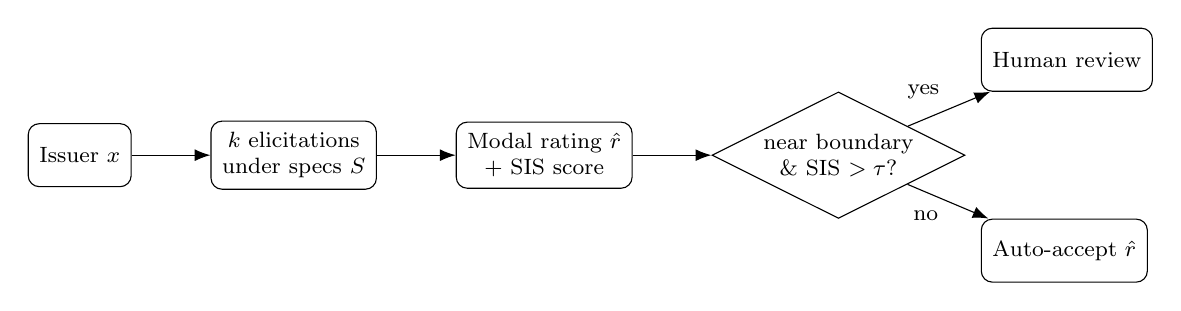
\begin{tikzpicture}[node distance=6mm and 10mm, font=\footnotesize,
 box/.style={draw, rounded corners, align=center, inner sep=4pt, minimum height=8mm},
 dec/.style={draw, diamond, aspect=2, align=center, inner sep=1pt},
 >={Latex[length=2mm]}]
\node[box] (issuer) {Issuer $x$};
\node[box, right=of issuer] (elicit) {$k$ elicitations\\under specs $S$};
\node[box, right=of elicit] (score) {Modal rating $\hat{r}$\\+ SIS score};
\node[dec, right=of score] (check) {near boundary\\\& SIS $>\tau$?};
\node[box, above right=4mm and 10mm of check] (review) {Human review};
\node[box, below right=4mm and 10mm of check] (pass) {Auto-accept $\hat{r}$};
\draw[->] (issuer) -- (elicit);
\draw[->] (elicit) -- (score);
\draw[->] (score) -- (check);
\draw[->] (check) -- node[above left]{yes} (review);
\draw[->] (check) -- node[below left]{no} (pass);
\end{tikzpicture}
\caption{Governance workflow. Each issuer is elicited $k$ times; the modal rating and specification-instability
score are recorded; issuers that are both near a consequential boundary and unstable are routed to review.}
\label{fig:governance}
\end{figure}

\section{Discussion}
We evaluate whether an LLM-generated credit rating can be treated as a stable assessment of a firm's
financial health or whether it depends heavily on how that measure is elicited. The main finding of the
pre-registered specification curve is that substantial instability remains even after controlling for the
underlying financial information. As expected, firm characteristics explain most of the total variation
in ratings, but the residual variation due to elicitation is large enough to change economically
meaningful decisions.

The variance decomposition clarifies the origin of this instability, and its interpretation is important.
No single controllable design choice explains more than $\sim$5\% of rating variance. Of the $\sim$25\%
OLS residual, only about 8\% is pure run-to-run seed variation; the rest is not identified as to
source under this resolution-limited design and is reported descriptively. The headline stability
conclusions do not depend on this decomposition. Under the descriptive main-effects decomposition no
measured main-effect share dominates; because interactions are not separately identified, this should not
be read as establishing that no individual design choice or interaction can have a larger causal effect.
The instability is nonetheless not dismissible as mere sampling noise (pure-seed variance is a minority of
the residual), and the headline flip and agreement results are model-free.

It is useful to separate two kinds of risk this induces, because they call for different controls.
\emph{Build-time} risk is the one-time consequence of fixing a particular provider, model snapshot, and
prompt template when a system is designed: under the descriptive main-effects decomposition no individual
design axis accounts for more than about 5\% of variance (these shares are not identified causal effects) and the
provider$\times$item interaction is non-negligible, so the chosen configuration selects a point on the
specification curve that need not generalize to other defensible configurations. \emph{Run-time} risk is
the ongoing 8.1\% pure seed variation that recurs on every call even with the configuration held fixed.
The two map to different mitigations, build-time risk is managed by evaluating across specifications
before deployment (the specification-instability score of Section~\ref{sec:sis}), run-time risk by
aggregating repeated calls (self-consistency, Section~\ref{sec:selfcons}), and to different lines of a
supervisory model-risk framework such as SR~11-7, one concerning model selection and validation, the
other ongoing monitoring.

The real-issuer experiment complements, rather than substitutes for, this identification strategy.
Crucially, it first demonstrates that direct evaluation on anonymized real firms is not automatically
clean: a model identifies around 22\% of the unperturbed issuers from financial information alone. After
issuer-specific scaling and screening, the fingerprint rate falls to 2.9\%, and substantial
specification variation is still observed. The real-issuer arm is therefore treated as an illustrative
descriptive check; its sample size does not support quantitative equivalence with the controlled battery.

\subsection{Mitigating exact-figure recognition in real-issuer evaluations}
The fingerprinting result also has implications beyond the credit-rating experiment at hand. Public
companies' financial information is widely disseminated and may have been included in the training data
of general-purpose LLMs. Removing company names does not necessarily remove issuer identity from an
evaluation: if a model can infer the issuer from the precise financial numbers, then a judgment that
appears to be based on the inputs may also draw on memorized information about that company. Perturbation
combined with explicit identification testing is a practical way to mitigate this risk when evaluating
LLMs on public financial entities.

Taken together, the results suggest that a credit rating produced by an LLM should not be interpreted as a
specification-invariant point estimate. Each response is one realization from a broader distribution
induced by the elicitation procedure. This does not imply that LLMs cannot contribute to credit analysis,
and the present study does not assess whether their ratings are more or less accurate than established
credit-assessment methods. Rather, a prerequisite for reliable use is to characterize the uncertainty
associated with reasonable elicitation choices before treating a point rating as a stable model output.

\subsection{Limitations}
These findings have several limitations that bound their scope. First, the study considers two model
providers and the specific model snapshots and configurations included in the pre-registered design
(Table~\ref{tab:models}); the results should therefore be viewed as evidence of how the evaluated systems
behave, not as a universal numerical estimate for all current or future LLMs. Relatedly, the evaluated
snapshots are each provider's low-cost (\texttt{nano}/\texttt{flash}) tier rather than a frontier model.
We study this tier deliberately, because cost pressure makes it the realistic choice for high-volume,
per-issuer credit screening. The concern that specification sensitivity might attenuate at the frontier
is examined in Section~\ref{sec:tier}: on the same grid, flagship models
(\texttt{gpt-5.4}, \texttt{gemini-3.1-pro-preview}) show an IG/HY flip statistically indistinguishable
from the nano/flash tier. We interpret this as not detecting attenuation (wide interval, absence of evidence
result) rather than as proof that scale does not matter; the reasoning-architecture arm
(Section~\ref{sec:reasoning}) also shows specification sensitivity remains in another model
class. The flagship comparison is based on one model per provider on a reduced grid, and a fuller frontier
sweep remains a useful extension.

Second, the main identification sample is a fixed 90-item constructed battery, with 45 profiles in the
credit-health task and 45 in the directional task. Repeated specifications increase coverage of the
elicitation space but not the number of independent underlying firm profiles, so the flip rates and
variance estimates remain sample statistics for the 45 credit-health items considered; we report
profile-clustered confidence intervals throughout to make this uncertainty explicit.

Third, the real-firm arm comprises 31 U.S. mid-cap business-to-business issuers selected under the
perturbation-and-fingerprint-screening design. This sample explores external validity descriptively but is much smaller than the
controlled battery at the relevant strata. The WATCH-stratum sample is small, and quantitative equivalence
between the real and constructed estimates is not established.

Fourth, the study measures stability, not absolute credit-rating capability. The Altman Z$''$ mapping
provides a pre-specified accounting-based benchmark for constructing and evaluating the controlled
credit-health battery, while disclosed agency ratings provide an alternative descriptive reference;
neither is treated as a unique ground-truth credit opinion. Whether generative models can produce more
accurate credit assessments than established statistical, market-based, or agency methods is a separate
research question.

A further methodological caveat concerns the variance decomposition. The 32-specification grid is a
balance-constrained D-optimal fraction chosen to make the main effects mutually near-orthogonal, but with
$N$ not divisible by the strength-2 requirement the design is resolution-limited: main effects can be
partially aliased with two-factor interactions. We therefore read the decomposition main-effects-first
and report the structured portion of the residual as ``unmodeled interactions'' rather than attributing
it to specific axes; the headline stability results (flip shares, agreement) are model-free and do not
depend on the ANOVA partition.

Within these bounds, the main stability finding is robust across the specification curve, the
temperature-0-honored subgrid, the provider comparison, and the rating-resolution analysis, and is further
illustrated descriptively by the perturbed and fingerprint-screened real-firm arm.

\subsection{Future directions}
The present design suggests several extensions. Larger and sector-stratified real-issuer samples would
yield more precise estimates of how specification instability varies with firm characteristics and
distance from rating boundaries. Similar designs could test retrieval-augmented or tool-using credit
agents, where access to external information may reduce some forms of uncertainty while adding further
specification choices. The proposed specification-instability score could be calibrated against downstream
decision quality and integrated into human-in-the-loop workflows. More broadly, the perturbation-and-fingerprint-screening
procedure could be applied to other evaluations of financial LLMs involving publicly documented entities:
explicitly testing whether an ostensibly anonymized case remains identifiable, in tasks such as risk
assessment, valuation, investment recommendation, and supervisory analysis, may help separate independent
reasoning from memorized entity knowledge.

Overall, reproducibility in AI-assisted credit assessment cannot be taken for granted from a single
elicitation. We present these findings as a case study of the evaluated systems rather than as a universal
numerical constant. Across a pre-registered specification curve, firm fundamentals explain most of the total
variation in machine-generated ratings, but substantial specification-level instability remains after
controlling for the underlying financial information, only a minority of which is pure run-to-run noise.
For the systems studied here, the elicitation procedure is part of the measurement: unless stability with
respect to reasonable elicitation choices has been demonstrated, a machine-generated credit rating should
not be treated as a specification-independent point estimate, and the specification-instability score offers
a concrete way to report that uncertainty.

\section{Methods}
\subsection{Design, battery, and benchmark}
The study is designed to measure \emph{elicitation stability}: whether an LLM produces a credit
assessment that is consistent when the underlying financial information is held constant but reasonable
choices in how the assessment is elicited vary. The aim is therefore not to estimate rating accuracy on a
naturally occurring population of firms, but to isolate variation attributable to the elicitation
process.

We use a constructed battery as the main identification environment because it allows firm fundamentals
to be held fixed while the elicitation specification varies, permits balanced representation across
credit-health conditions, and provides a benchmark that can be computed before any model is queried.
Restricting the analysis to public companies would introduce a further source of uncertainty,
because an LLM might identify an issuer from financial information it was exposed to during training. We
therefore use the controlled battery for the main analysis and a separately perturbed and fingerprint-screened real-firm
sample for a complementary descriptive external-validity check.

The battery consists of 90 fixed firm-quarter profiles. Each profile is summarized in a compact financial
statement, including revenue, EBIT, total assets and liabilities, equity, working-capital figures, and
retained earnings. The profiles comprise two equally sized task families: 45 credit-health items, for
which the model produces a credit rating, and 45 directional items, for which the model produces a
buy/hold/sell call. All analyses in this paper use the 45 credit-health profiles; the 45 directional
profiles are part of the pre-registered battery but are not analyzed here.

For the credit-health task, each profile is associated with a pre-specified Altman Z$''$ accounting-based
reference \citep{altman1968}, computed with coefficients 6.56, 3.26, 6.72, and 1.05 and cutoffs 2.60 and
1.10 (Z$''\ge2.60$ = safe, $1.10<{}$Z$''<2.60$ = watch, Z$''\le1.10$ = distress). The resulting safe,
watch, and distress strata each contain 15 observations, evenly distributed across the 45 credit-health
profiles. The machine's letter rating is mapped deterministically to notch, three-band, and IG/HY
outcomes as in Table~\ref{tab:map}; the Altman mapping provides a deterministic accounting reference for
constructing and stratifying the controlled battery and is not treated as a unique ground-truth agency
rating, because our interest is stability across elicitation specifications rather than absolute rating
accuracy. The benchmark and battery were frozen under a pre-registration hash before any model query, and
an independent post-hoc re-execution from the frozen financial facts reproduces all 45 benchmark
classifications.

\begin{table}[t]\centering
\caption{Deterministic mapping from the machine letter rating to coarser resolutions, and the Altman
Z$''$ benchmark strata. The three-way band and the IG/HY split share the same investment-grade cut.}
\label{tab:map}
\begin{tabular}{llll}\toprule
Letter grade & Notch & Three-way band & IG/HY \\\midrule
AAA & AAA & SAFE & Investment grade \\
AA$+$ & AA & SAFE & Investment grade \\
AA & AA & SAFE & Investment grade \\
AA$-$ & AA & SAFE & Investment grade \\
A$+$ & A & SAFE & Investment grade \\
A & A & SAFE & Investment grade \\
A$-$ & A & SAFE & Investment grade \\
BBB$+$ & BBB & SAFE & Investment grade \\
BBB & BBB & SAFE & Investment grade \\
BBB$-$ & BBB & SAFE & Investment grade \\\midrule
BB$+$ & BB & WATCH & High yield \\
BB & BB & WATCH & High yield \\
BB$-$ & BB & WATCH & High yield \\
B$+$ & B & WATCH & High yield \\
B & B & WATCH & High yield \\
B$-$ & B & WATCH & High yield \\\midrule
CCC$+$ & CCC & DISTRESS & High yield \\
CCC & CCC & DISTRESS & High yield \\
CCC$-$ & CCC & DISTRESS & High yield \\
CC & CC & DISTRESS & High yield \\
C & C & DISTRESS & High yield \\\bottomrule
\end{tabular}

\vspace{3pt}
{\footnotesize\raggedright The notch resolution drops the $+$/$-$ modifiers, collapsing
the 21 letter grades to 9 notches. \emph{Altman Z$''$ strata:} SAFE $\ge 2.60$;
WATCH $1.10$--$2.60$; DISTRESS $\le 1.10$.\par}
\end{table}

\subsection{Specification grid and data collection}
We manipulate seven researcher-controlled elicitation dimensions: model provider (OpenAI, Google), model
version (a current and a prior snapshot per provider), temperature (0 or 1.0), prompt paraphrase (three
semantically equivalent formulations), output format (JSON or free-text), few-shot exemplars (zero or
two), and answer presentation (original prose versus a table with reversed option ordering). The exact
model snapshots and the collection window are listed in Table~\ref{tab:models}. A balance-constrained
D-optimal fractional grid was generated from an effect-coded main-effects model with the design seed
frozen in advance; the two-provider portion used here comprises 32 specifications, each evaluated over
three seeds. Provider metadata were preserved as returned, including effective generation settings where
available; the requested temperature of 0 was not uniformly honored by providers.

The confirmatory experiment therefore comprises $90\times32\times3=8{,}640$ elicitation cells
($4{,}320$ on the 45 credit-health profiles), of which 8{,}633 returned substantive content. The seven
non-substantive cells (empty or unparseable responses, $0.08\%$) are dropped listwise: they enter no
agreement, flip, or variance computation, and because every statistic is an average over the cells that
did parse, their omission cannot manufacture instability. Each call is stored as an immutable JSON record
containing the experimental specification, the returned content, and the available provider metadata.
Data collection and analysis are separated: all confirmatory analyses run only on the frozen response
corpus and do not re-query any model.

\begin{table}[t]\centering
\caption{Model snapshots evaluated. The four confirmatory snapshots (two providers, current and prior
each) constitute the main $8{,}640$-cell experiment; the two flagship snapshots are the separate
model-tier robustness arm (Section~\ref{sec:tier}). Responses were collected once and frozen; all
reported results reproduce offline from the frozen corpus.}\label{tab:models}
\begin{tabular}{lll}\toprule
Provider & Model snapshot & Role \\\midrule
OpenAI & \texttt{gpt-5.4-nano} & current (confirmatory) \\
OpenAI & \texttt{gpt-5-nano-2025-08-07} & prior (confirmatory) \\
Google & \texttt{gemini-3.5-flash} & current (confirmatory) \\
Google & \texttt{gemini-2.5-flash} & prior (confirmatory) \\\midrule
OpenAI & \texttt{gpt-5.4} & flagship (robustness) \\
Google & \texttt{gemini-3.1-pro-preview} & flagship (robustness) \\
DeepSeek & \texttt{deepseek-r1} (OpenRouter) & reasoning (robustness) \\\bottomrule
\end{tabular}

\vspace{3pt}
{\footnotesize\raggedright The four confirmatory snapshots were queried once in the frozen
confirmatory run (July 2026); the two flagship snapshots in the later robustness run (August 2026); and the reasoning
snapshot (\texttt{deepseek-r1}, served via the OpenRouter API) in a separate reasoning run (September 2026). All were
used offline thereafter; aliases without an embedded date stamp are pinned by these query months, with the exact dates recorded in the frozen manifests. The
reasoning model is API-served, so its temperature and seed are request parameters, not self-hosted determinism.}
\end{table}

\subsection{Outcome construction and statistical analysis}
Stored model responses are parsed under three rules, strict, lenient, and tolerant, applied after
collection. Credit ratings are first expressed on the full 21-grade letter scale and then
deterministically aggregated into notch categories, three broad credit bands, and the binary
investment-grade/high-yield classification (Table~\ref{tab:map}). This permits examination of stability at
increasingly coarse rating resolutions without additional model calls.

Agreement across specifications is measured with Fleiss' $\kappa$. Within- and cross-provider agreement
is computed on matched firm profiles and seeds. Variation in the full letter-rating rank is decomposed by
ordinary least squares with Type-II analysis of variance, with terms for the underlying item, the
elicitation-design dimensions, the provider-by-item interaction, and a residual. To interpret the
residual, we additionally estimate the \emph{pure within-cell seed variance} as the sum of squares across
the three seeds within each identical item$\times$specification cell, divided by the total sum of squares;
the difference between the OLS residual and this pure-seed component is reported as ``other unexplained''
(unmodeled interactions).

All analyses are pre-registered unless labelled post-hoc, and inference uses distribution-free resampling
throughout, so no normality assumption is made. Uncertainty for the main quantities is estimated by
profile-clustered percentile bootstrap resampling over the underlying firm profiles, instead of over
individual model calls, thereby preserving dependence among repeated elicitations of the same profile; we
report the variance shares (item and pure-seed) and the IG/HY flip rate with
two-sided 95\% confidence intervals (2{,}000 replicates for the flip rate, 1{,}000 for the
variance-share and specification-curve quantities). Specification invariance under the temperature-0-honored
setting is tested on the provider-setting combination whose metadata confirm that temperature was
honored (Google at temperature 0). We test a rating-invariance null: specification-condition assignments
are permuted across profiles (rather than permuting accuracy labels), and the statistic is the
between-specification spread of the item-centred letter rating, compared with the distribution generated
by $2{,}000$ such permutations in a one-sided test, $p=(k{+}1)/(n{+}1)$, where $k$ is the number of
permuted statistics at least as extreme as observed and $n=2{,}000$. The test is one-sided in that only an
observed spread greater than the permutation distribution provides evidence against specification
invariance. The real-firm arm is presented descriptively: the real-firm and constructed-battery
WATCH-stratum flip shares are compared by their issuer-clustered bootstrap difference and interval, with
no equivalence claim. The significance threshold is $\alpha=0.05$ for all
formal tests. To mitigate the risk of selective reporting within the specification multiverse, we
pre-registered the estimands and specification grid and report the entire specification curve rather than
a selected subset. We reserve ``significant'' for results accompanied by a $p$-value and otherwise use
``substantial'' or ``considerable.''

For the binary IG/HY outcome, the per-comparison flip probability is computed separately for each
credit-health profile from its observed distribution of ratings across the entire elicitation grid, so
that two elicitations may differ on any specification dimension or seed. The resulting pair falls on
opposite sides of the IG/HY boundary with probability equal to one minus the Gini--Simpson concentration
of the profile's binary labels, and the reported flip rate is the average of this quantity over the 45
credit-health profiles. The same per-issuer quantity, reported at the decision resolution of interest, is
the specification-instability score developed in Section~\ref{sec:sis}.

The revision is supported by three post-hoc analyses, which are run offline from the frozen corpora. The
specification-instability score is validated on a 16/16 held-out-specification split with an operating
threshold selected by Youden's $J$ (reported descriptively); the range of variance explained by the
elicitation axes is described in a main effects model, a main plus two-way interaction model, and an
issuer-out-of-sample regularized model; and the real-firm external-benchmark specification curve is tested
with an issuer-preserving permutation (specification labels permuted within issuer). The
reasoning-architecture arm (Section~\ref{sec:reasoning}) is frozen under \texttt{MANIFEST\_REASONING.sha256}.

\subsection{Real-firm arm}
To test the persistence of specification instability outside the constructed battery, we assemble a
complementary sample of 31 U.S. business-to-business issuers with market capitalizations between \$2
billion and \$15 billion whose most recent Form 10-K discloses a current long-term agency credit rating.
S\&P is the primary rating source; where S\&P ratings are unavailable, Moody's or Fitch ratings are
mapped to a common scale. Each rating is preserved with a verbatim filing quotation, a permanent SEC
document URL, and a document hash.

Because these figures are publicly reported by real issuers, there is a risk of contamination if a model
can identify a company. We therefore first perform a pre-registered fingerprinting test in which the
models are asked to identify issuers from anonymized financial profiles; Gemini-Flash identifies about
22\% of the selected issuers from the original figures, confirming that removing the company name does not
guarantee independence from memorized issuer information. To reduce this risk, every dollar-denominated
quantity for an issuer is multiplied by a single issuer-specific factor sampled from a log-uniform
distribution over $[0.6,1.7]$. The same factor applies to all monetary amounts, so the credit-health
analysis retains the financial-ratio structure while disrupting exact-figure lookup. We also
exclude consumer-facing companies to reduce recognition from highly distinctive public profiles. The
fingerprint-identification rate falls to 2.9\% after perturbation, below the pre-registered 5\%
fingerprint-identification threshold.

Each retained perturbed issuer is then scored on a fixed 12-specification grid spanning presentation,
provider, prompt paraphrase, and output format, at three seeds, and the constructed battery is re-scored
under the same grid for a matched comparison on the WATCH stratum. This arm uses disclosed agency ratings
as a descriptive real-world reference; the primary comparison is stability across specifications.

\subsection{Reproducibility}
The entire experimental pipeline is archived so that the reported results can be reproduced without
further model calls. The frozen materials comprise the 90-item battery, the specification grid, the
prompt templates, the rating scale, the frozen response corpus, the analysis panel, the real-firm arm,
the analysis code, the generated outputs, and SHA-256 integrity manifests. The complete set of
confirmatory tables, figures, and reported statistics regenerates from a single offline entry point.
Provider API credentials are required only to collect new model responses and are not needed to reproduce
any result reported in this study.

\section*{Declaration of generative AI and AI-assisted technologies in the manuscript preparation process}
Generative AI was used to assist with grammar correction and minor language edits of the authors' own
text, and with software scaffolding, development, and coding of the analysis and reproducibility pipeline
(Anthropic Claude), in all cases under the authors' direction. Separately, large language models are the
object of study in this work, the credit-rating elicitations under analysis, as described above; every
such elicitation is recorded in the specification grid and frozen corpus. The authors reviewed and
verified all such output and take full responsibility for the content.


\section*{Declaration of competing interest}
S.C. and R.C. each declare no competing interests.

\section*{Funding}
This research received no external funding.

\section*{Ethics}
This study did not involve human participants, human tissue, or animal subjects, and used no personally
identifiable or sensitive personal data; ethical approval was therefore not required. The analysis uses
only synthetic firm profiles, publicly available corporate financial disclosures (SEC filings), and the
authors' own model elicitations.

\section*{Data availability}
All data and code required to reproduce the study are openly available in a deterministic, offline
reproducibility capsule (MIT license) provided as anonymized supplementary material with this submission;
the public repository and its citable DOI are withheld here for double-blind review and will be provided
on acceptance.
Within the capsule, \texttt{data/frozen/main/} contains the pre-registered 90-item firm battery
(\texttt{battery\_90.json}; 45 credit-health $+$ 45 directional items), the specification grid, the prompt
paraphrases, and the rating scale; \texttt{data/raw/main/} holds the frozen
response corpus; \texttt{data/panel/panel.parquet} is the analysis panel; and
\texttt{data/frozen/realarm/} with \texttt{data/raw/realarm/} contain the perturbed and fingerprint-screened real-firm arm
(anonymized perturbed battery, sealed issuer crosswalk, rating provenance with verbatim 10-K quotation,
permanent SEC URL, and document hash per issuer, and the arm/comparator/fingerprint model-output panels).
The flagship model-tier arm (\texttt{gpt-5.4} $+$ \texttt{gemini-3.1-pro-preview} on the frozen
12-specification grid) is in \texttt{capture/flagship\_runs/}, fixed by \texttt{MANIFEST\_FLAGSHIP.sha256};
the reasoning-architecture arm (\texttt{deepseek-r1} on the same grid) is in \texttt{capture/reasoning\_runs/},
fixed by \texttt{MANIFEST\_REASONING.sha256}.
Analysis code is in \texttt{analysis/}, outputs and figures in \texttt{results/}, and SHA-256 manifests in
\texttt{manifest/}. A single offline entry point, \texttt{reproduce.sh}, regenerates every reported
number, table, and figure, with no model calls and no API keys. A self-contained companion,
\texttt{REPRODUCIBILITY\_DOCUMENTATION.pdf} (provided with this submission), documents the
complete archive---data inputs and provenance, every analysis script and its outputs, the one-command
reproduction, the verification and determinism procedure, and the pinned environment---so that the study
can be understood and re-run from that single file. The underlying SEC filings (Form 10-K and
company-facts XBRL) are publicly available through the SEC EDGAR system.

\bibliographystyle{cas-model2-names}
\bibliography{references}

\end{document}
